\section{Elektrische Netzwerke, Systeme}
\tikzsetexternalprefix{compiledFigures/elektrischeNetzwerke/}
\index{Elektrische Netzwerke|see{Elektrische Systeme}}
\index{Elektrische Systeme}
Skript Herr Neubauer Seite 36-37.
Netzwerk-Klassifizierung


\subsection{Netzwerk-Klassifizierung}
\index{Elektrische Systeme!Klassifizierung}
\paragraph{Auflösung}
\index{Elektrische Systeme!Klassifizierung!Auflösung}
\begin{tabular}{|l|l|l|}
	\hline
	& kontinuierlich & diskret \\
	\hline
	Elemente & räumlich verteilt & konzentriert \\
	\hline
	Signal-Änderung & zeitlich stetig & intervall-bedingt\\
	& wertmässig analog & digital\\
	\hline
\end{tabular}
\paragraph{Netzwerk-Elemente}
\index{Elektrische Systeme!Klassifizierung!Elemente}
R-, RC-, RL-, RLC-Netzwerke
\paragraph{Ein- und Ausgänge}
\index{Elektrische Systeme!Ein-/Ausgänge}
\begin{tabular}{llll}
Bezeichnung & Eintor=Zweipol & Zweitor=Vierpol & N-tor=2N-pol \\
Zweigpaare & 1 & 2 & N\\
\end{tabular}\\
\ldots führen aus dem elektrischen Netzwerk heraus.
\paragraph{Verwendung}
Filter, Regelsysteme, Signalformer, Nachrichtensysteme, Niederspannungsnetze
u.a.
\paragraph{Systemeigenschaften}
\index{Elektrische Systeme!Klassifizierung!Eigenschaften}
Aktiv – passiv, linear – nichtlinear, zeitvariant – zeitinvariant,
ohne Speicher – mit Speicher, minimalphasig – nicht minimalphasig\\


Die allgemeine Theorie der elektrischen Netzwerke begründet sich auf Arbeiten von Foster,
Cauer, Brune, Bode, Darlington, Piloty, Bader, Guillemin, Wagner, Heaviside und anderen.

\subsection{Dualität}
\index{Elektrische Systeme!Dualität}
\index{Elektrische Systeme!Dualität!Zweipole}
\subsubsection{Duale Zweipole}
$\rightarrow$ vertauschte Rollen von Spannung und Strom\\
\begin{tabular}{llll}
$u=L\frac{di}{dt}$&$ \leftrightarrow$&$ i=C\frac{du}{dt}$
& L und C sind zueinander dual\\
$u=R\cdot i $&$ \leftrightarrow $&$ i=G\cdot u$ &
R und G sind zueinander dual\\
$U_q $&$ \leftrightarrow $&$ i_q $
& Strom- und Spannungsquellen sind dual\\
\end{tabular}

\subsubsection{Duale Schaltungen}
\index{Elektrische Systeme!Dualität!Schaltung}
Werden durch Gleichungen mit derselben "`mathematischen Struktur"' beschrieben.
Alle Ströme im einen Netzwerk sind proportional zur entsprechenden Spannung im
andern Netzwerk und umgekehrt.\\
Aus $\Sigma I=0$ wird $\Sigma U=0$ und umgekehrt\\
Aus Serieschaltungen werden Parallelschaltungen und umgekehrt\\
Aus Knoten werden Maschen und umgekehrt\\
\paragraph{Beispiel}
\begin{figure}[!ht]
\centering
\subfloat[Serieschaltung]{
	\tikzexternaldisable
\begin{circuitikz}[scale=2, european, american inductors]
\ctikzset{voltage/european label distance=3}
\ctikzset{bipoles/length=1.2cm}
	\draw (0,0) to[american voltage source, label=\mbox{$U_q=60V$}] (0,2)
	to [short, i=\mbox{$I=0.2$}] (2,2)
	to [R, label=\mbox{$R_1=100\Omega$}] (2,1)
	to [R, label=\mbox{$R_2=200\Omega$}] (2,0)
	-- (0,0)
	;
	\draw (1.9,2) to[open, v>=\mbox{$U_1=20V$}] (1.9,1);
	\draw (1.9,1) to[open, v>=\mbox{$U_2=40V$}] (1.9,0);
\end{circuitikz}
\tikzexternalenable

	\label{fig:elNetzwerke:Serieschaltung}
}
\qquad
\qquad
\subfloat[Parallelschaltung]{
	\begin{circuitikz}[scale=2, european, american inductors]
\ctikzset{voltage/european label distance=3}
%\ctikzset{bipoles/length=1.2cm}
	\draw (0,0)	to[american current source, label=\mbox{$I_q'=0.2V$}] (2,0)
	-- (2,-2)
	to [R, l_=\mbox{$G_2'=200S$}] (1,-2) 
	to [short, i_=\mbox{$I_2'=40A$}] (0,-2)
	-- (0,0);
	\draw (2,-1) to [R, label=\mbox{$G_1'=100S$}] (1,-1)
	to [short, i_=\mbox{$I_1'=20A$}] (0,-1);
	\draw (0,-0.12) to [open, v_<=\mbox{$U'=0.2V$}] (2,-0.12);
\end{circuitikz}

	\label{fig:elNetzwerke:Parallelschaltung} 
}
\caption[Serie- und Parallelschaltung]{Serie- und Parallelschaltung}
\label{fig:elNetzwerke}
\end{figure}

\begin{tabular}{ll}
Serieschaltung & Parallelschaltung \\
$U_1+U_2=U_q$
& $I_1'+I_2'=I_q'$\\ $U2=Uq\frac{R_2}{R_1+R_2}$ & $I_2'=I_q'\frac{G_2'}{G_1'+G_2'}$\\
\end{tabular}

\subsubsection{Dualfaktor D}
\index{Elektrische Systeme!Dualfaktor}
Anpassung des Impedanzlevels, z.B.\\
alle Ströme $:1000$,\\
alle Spannungen $x1000$\\
$\rightarrow$ alle Widerstände (Imped.) $x10^6$\\
$\rightarrow$ alle Leitwerte (Admitt.) $:10^6$\\
Berechnung der dualen Grössen:\\
\begin{align}
	I_q'&=\frac{U_q}{1000\Omega }\nonumber\\
	U'&=I\cdot 1000\Omega \nonumber\\
	G'&=\frac{R}{\left(1000\Omega\right)^2}\nonumber\\
	R'&=G\left(1000 \Omega\right)^2\nonumber
\end{align}
$1000 \Omega =$ Dualfaktor D, kann beliebig gewählt werden\\
\begin{tabular}{ll}
	$L \leftrightarrow C^2$ & $\underline{Y}'=\frac{\underline{Z}}{D^2}$\\
	& $j\omega C'=\frac{j \omega L}{D^2} \Rightarrow C'=\frac{L}{D^2}$\\
	& $L'=C\cdot D^2$
\end{tabular}\\
Skript Seite 37\\

Skript Seite 39: Finden der dualen Schaltung\\

\subsection{Netzwerkfunktionen}
\index{Elektrische Systeme!Netzwerkfunktionen}
\index{Netzwerkfunktionen}

\begin{tabular}{p{0.08\textwidth}p{0.85\textwidth}}
	\textbf{bisher:} & $j\omega$, gelegentlich abgekürzt mit $p=j\omega$ \\
	\textbf{neu:} & komplexe Frequenz $p=\sigma + j \omega$ (Erweiterung). Statt p
	wird oft auch s verwendet ($\rightarrow$ Laplace Transformationen)	\\
\end{tabular}

%\usepackage{graphics} is needed for \includegraphics
\begin{figure}[htp]
\centering
  \subfloat[p-Ebene]{
  	\label{fig:ElNetzw:pEbene}
  	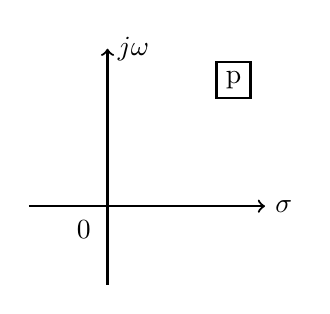
\begin{tikzpicture}[thick, ->]
  \draw (-1,0) -- +(3,0) node[right] {$\sigma$};
  \draw (0,-1) -- +(0,3) node[right] {$j \omega$};
  \node at (-0.3,-0.3) {0};

  \node[draw] at  (1.6,1.6) {p};
\end{tikzpicture}
  }
  \qquad
  \subfloat[Zeiger]{
    \label{fig:ElNetzw:ZeigerDiag}
    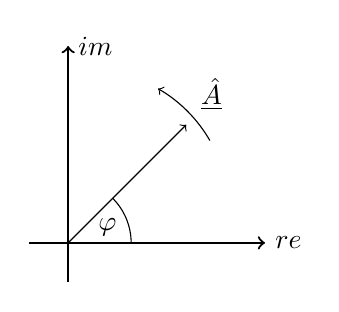
\begin{tikzpicture}
\begin{scope}[thick, ->]
  \draw (-0.5,0) -- +(3,0) node[right] {$re$};
  \draw (0,-0.5) -- +(0,3) node[right] {$im$};
\end{scope}

  \draw (0.8,0) arc (0:45:0.8);
  \node at (0.5,0.2) {$\varphi$};
  \draw [->] (0,0) -- (1.5,1.5) node[above right=1.8] {$\underline{\hat{A}}$}; 
  \draw[->] (1.8,1.3) arc (30:60:1.8);
\end{tikzpicture}
  }
  \caption[p-Ebene und Zweigerdiagramm]{p-Ebene und Zweigerdiagramm}
  \label{fig:ElNetzw:pEbeneZeigerDiag}
\end{figure}

\textbf{Bedeutung:}\\
\begin{tabular}{ll}
	\textbf{bisher:} & $a(t)=Re\{\underline{a}(t)\}=Re\{\hat{A}\cdot e^{j\phi}\cdot
	e^{j\omega t}\}$ \\
	& $\rightarrow \text{Sinussignal: } a(t)=\hat{A}\cdot\cos{\left(\omega t +
	\phi\right)}$\\ mit $p=\sigma+j\omega$ & $a(t)=Re\{\hat{A}\cdot e^{j\phi}\cdot
	e^{\sigma t}\cdot e^{j\omega t}\}$\\
	& $a(t)=\hat{A}\cdot e^{\sigma t} \cdot \cos{\left(\omega t + \phi\right)}$\\
\end{tabular}\\
Sinussignal, das exponentiell abklingt $(\sigma < 0)$ oder exponentiell
anschwillt $(\sigma > 0)$. Für $\sigma = 0$ verhält es sich wie "`früher"'.\\
\begin{itemize}
  \item Komplexe Rechnung gilt auch für $p=\sigma+j\omega$\\
  \item Wird ein lineares Netzwerk mit $a_q=\hat{A}\cdot e^{\sigma t}
  \cos\left(\omega t + \phi\right)$ angeregt, sind alle Ströme und Spannungen
  auch exponentiell abklingend oder anschwillend.
\end{itemize}
Skript Seiten 39 bis 43, Netzwerkfunktionen

\subsection{P-N-Plan, P-N-Diagramm}
\index{Pol-Nullstellen Diagramm}
\index{P-N-Diagramm|see{Pol-Nullstellen Diagramm}}
\index{P-N-Plan|see{Pol-Nullstellen Diagramm}}
\textbf{Bsp} Tiefpass 1. Ordnung\\
$\underline{F}(p)=\frac{\underline{U}_2}{\underline{U}_1}=\frac{\frac{1}{pC}}{R+\frac{1}{pC}}=\frac{1}{pRC+1}
=\frac{1}{RC\left(p+\frac{1}{RC}\right)}=F_0\frac{1}{p-p_1}$\\
\begin{tabular}{ll}
Nullstellen: & keine\\
Pole: & $pRC+1=0$ \\
& $p=-\frac{1}{RC}=p_1$\\
\end{tabular}\\
\begin{figure}[htp]
\centering
  \subfloat[RC-Tiefpass]{
    \begin{circuitikz}[scale=2, european, american inductors]
\draw (0,0) to [R, l=$R$, *-*] (1,0)
	to [short, -*] (2,0);
\draw (1,0) to [C, l=$C$, *-*] (1,-1);
\draw (0,-1) to [short, *-*] (2,-1);
\draw (0,0) to[open, v>=$U_1$] (0,-1);
\draw (2,0) to[open, v^>=$U_2$] (2,-1);
\node at (0,-1.5) {};
\end{circuitikz}
    \label{fig:ElNetzw:Bsp1:RCTiefpass}
  }
  \qquad
  \subfloat[Pol-Nullstellen Diagramm]{
    \usepgflibrary{shapes.misc}
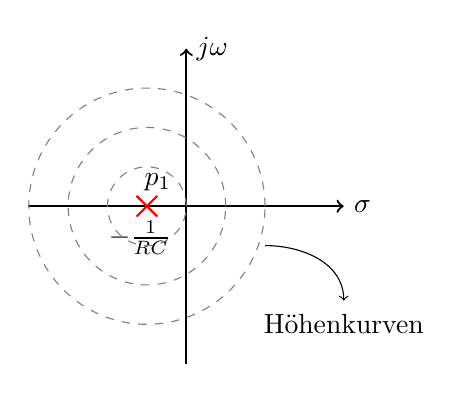
\begin{tikzpicture}
\begin{scope}[thick, ->]
  \draw (-2,0) -- +(4,0) node[right] {$\sigma$};
  \draw (0,-2) -- +(0,4) node[right] {$j \omega$};
\end{scope}
 
  \node[cross out, draw=red, thick] at (-0.5,0) {}
     node[below left=2] {$- \frac{1}{RC}$}
     node[above left=2] {$p_1$};

\draw[dashed, color=gray](-0.5,0) circle (1);
\draw[dashed, color=gray](-0.5,0) circle (0.5);
\draw[dashed, color=gray](-0.5,0) circle (1.5);
\draw (1,-0.5) edge[out=0, in=90, ->] (2,-1.2);
\node at (2,-1.5) {Höhenkurven};

\end{tikzpicture}
    \label{fig:ElNetzw:Bsp1:PolNullstellenDiag}
  }
  \caption[RC-Tiefpass und Pol-Nullstellen Diagramm]{RC-Tiefpass und
  Pol-Nullstellen Diagramm zum Beispiel}
  \label{fig:ElNetzw:PolNullstellenDiag}
\end{figure}
$F(p)=|\underline{F}(p)|=\frac{F_0}{|p-p_1|}$\\

\subsubsection{Zusammenhang Übertragungsfunktion und freier Schwingung}
\begin{figure}[htp]
\begin{center}
  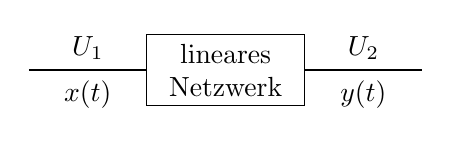
\begin{tikzpicture}

\draw[thick] (-1.5,0) -- +(1.5,0) 
  node[midway, above] {$U_1$}
  node[midway, below] {$x(t)$};

\node[text width = 2cm, text centered, inner xsep=0, draw] at (1,0) {lineares Netzwerk};

\draw[thick] (2,0) -- +(1.5,0) 
  node[midway, above] {$U_2$}
  node[midway, below] {$y(t)$};

\end{tikzpicture}
  \caption[Lineares Netzwerk]{Lineares Netzwerk}
  \label{fig:ElNetzw:LinNetzwerk}
\end{center}
\end{figure}
Homogene Lösung der DGL
\begin{align}
	\underline{F}(p)&=\frac{\underline{P}_n(p)}{\underline{Q}_m(p)}\nonumber\\
	\underline{F}(j\omega)&=\frac{P_n(j\omega)}{Q_m(j\omega)}\nonumber\\
	\underline{F}(j\omega)&=\frac{a_0+a_1j\omega+a_2(j\omega)^2+\ldots+a_n(j\omega)^n}{b_0+b_1j\omega+\ldots+b_m(j\omega)^m}=\frac{\underline{U}_2}{\underline{U}_1}\nonumber
\end{align}
Daraus folgt:
\begin{align}
\underline{U}_2(b_0+b_1j\omega+b_2(j\omega)^2+\ldots+b_m(j\omega)^m)=\underline{U}_1(a_0+a_1j\omega+a_2(j\omega)^2+\ldots+a_n(j\omega)^n)\nonumber
\end{align}

Wir erinnern uns: Komplexe Amplitude mit $j\omega$ multiplizieren
$\widehat{=}$ ableiten.\\
\begin{align}
	&\Rightarrow U_2(t)\cdot b_0 + \dot{U}_2b_1 +
	\ddot{U}_2b_2+\ldots+U_2^{(m)}\cdot
	b_m=a_0U_1(t)+a_1\dot{U}_1+a_2\ddot{U}_1+\ldots+a_nU_1^{(n)}\nonumber\\
	&\Rightarrow b_0U_2+b_1\dot{U}_2+b_2\ddot{U}_2+\ldots+b_mU_2^{(m)}=0\nonumber
\end{align}
Ansatz $U_2=\hat{U}_2\cdot e^{\alpha t}$\\
\begin{align}
	&\Rightarrow \underbrace{\hat{U}_2e^{\alpha t}}_{\neq 0}\underbrace{(b_0+\alpha
b_1+\alpha^2b_2+\ldots+\alpha^mb_m)}_{\text{charakteristische
Lösung: }\alpha_1, \alpha_2, \ldots \alpha_m}=0\nonumber\\
	U_{2h}&=c_1e^{\alpha_1t}+c_2e^{\alpha_2t}+\ldots+c_me^{\alpha_mt}\nonumber
\end{align}
$\Rightarrow$ Die Lösungen $\alpha_1\ldots\alpha_m$ der charakteristischen
Gleichung entsprechen den Nullstellen von $Q_m(p)$ bzgl den Polen von
$\underline{F}(p)$\\
\begin{align}
\alpha_i&=p_i\nonumber\\
\rightarrow
U_h(t)&=\hat{U}_{h1}e^{p_1t}+\hat{U}_{h2}e^{p_2t}+\ldots+U_{hm}e^{p_mt}\nonumber
\end{align}
$Re\{p_i\} \Rightarrow $ Dämpfungskonst $=\sigma_i\ (p<0)$\\
$Im\{p_i\}=$
Eigenfrequenz\\
Skript, Seite 49\\

\subsubsection{Fallunterscheidung}
\begin{itemize}
  \item siehe auch Abbildung \ref{fig:elNetzw:Fallunterscheidung}
  \item reeller Pol $p_i=\sigma_i \rightarrow$ ergibt Lösungsanteil
  $c_ie^{\sigma_it}$
  \item zweifacher reeller Pol $\rightarrow
  c_ie^{\sigma_it}+c_{i+1}te^{\sigma_it}$
  \item konjugiert komplexes Polpaar $p_{ij}=\sigma_i\pm j\omega i$
\end{itemize}
\begin{align}
  &\rightarrow \underline{c}_{i1}e^{(\sigma_i+j\omega
  i)t}+\underline{c}_{i2}e^{(\sigma_i-j\omega i)t}\nonumber\\
  &=e^{\sigma_it}\left(\underline{c}_{i1}e^{j\omega_it}+\underline{c}_{i2}e^{-j\omega_it}\right)\nonumber\\
  &\underline{c}_{i1}=c_ie^{j\varphi},
  \underline{c}_{i2}=c_ie^{-j\varphi}\nonumber\\
  &=e^{\sigma_it}\left(c_ie^{j\left(\omega_it+\varphi\right)}+c_ie^{-j\left(\omega_it+\varphi\right)}\right)\nonumber\\
  &=e^{\sigma_it}\cdot
  \underbrace{c_i\cdot2}_{=A}cos(\omega_it+\varphi)=Ae^{\sigma_it}cos(\omega_it+\varphi)\nonumber
\end{align}
$\sigma_i > 0$ exponentiell Ansteigend $\rightarrow$ instabil\\
$\sigma_i < 0$ exponentiell Abklingend $\rightarrow$ Pol in linker Halbebene\\

\begin{figure}[!ht]
\begin{center}
  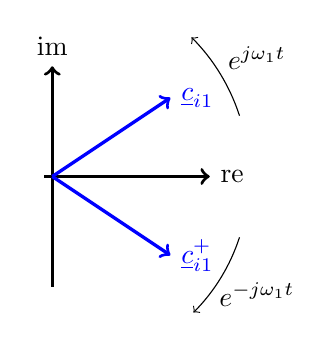
\begin{tikzpicture}
\begin{scope}[->, very thick]
  \draw (-0.1, 0) -- (2,0) node[right] {re};
  \draw (0,-1.4) -- (0,1.4) node[above] {im};
  \draw[blue] (0,0) -- (1.5,1) node[right] {$\underline{c}_{i1}$};
  \draw[blue] (0,0) -- (1.5, -1) node[right] {$\underline{c}_{i1}^+$};
\end{scope}

\draw[->] (2.3776,0.7725) arc (18:45:2.5) node at(30:3) {$e^{j\omega_1t}$};
\draw[->] (2.3776,-0.7725) arc (-18:-45:2.4) node at(-30:3) {$e^{-j\omega_1t}$};
\end{tikzpicture}

  \caption{Veranschaulichung zur Fallunterscheidung}
  \label{fig:elNetzw:Fallunterscheidung}
\end{center}
\end{figure}

\subsection{Parallel-SK}
\begin{figure}
	\centering
	\begin{circuitikz}[scale=2, european, american inductors]
\ctikzset{voltage/european label distance=3}
%\ctikzset{bipoles/length=1.2cm}
	\draw (0,-0.3) to [short, -*] (0,-0.5);
	\draw (-1,-0.5) -- (1,-0.5);
	\draw (0,-1.5) to [short, *-] (0,-1.7);
	\draw (-1,-1.5) -- (1,-1.5);
	\draw (-1,-0.5) to [L] (-1,-1.5);
	\draw (0,-0.5) to [C] (0,-1.5);
	\draw (1,-0.5) to [R] (1,-1.5);
\end{circuitikz}

  \caption[LCR Parallelschwingkreis]{LCR Parallelschwingkreis}
  \label{fig:ElNetzw:LCRParallelschwingkreis}
\end{figure}
$\underline{Z}(p)=\frac{1}{\frac{1}{R}+pC+\frac{1}{pL}}=\frac{pL}{1+p\frac{L}{R}+p^2LC}$\\
mit $\omega_r=\frac{1}{\sqrt{LC}}, Q=R\cdot\sqrt{\frac{C}{L}}$\\
%TODO nextline unterklammer Lomegar =K 
$\underline{Z}(p)=\omega_r^2\frac{pL}{p^2+\frac{\omega_r}{Q}p+\omega_r^2}=L\omega_r^2
\frac{p}{(p-\underline{p}_1)(p-\underline{p}_2)}$\\
Nullstelle: $\underline{z}_1=0$\\
Pole:
$p_{1,2}=\frac{-\frac{\omega_r}{Q}\pm\sqrt{\frac{\omega_r^2}{Q^2}-4\omega_r^2}}{2}=-\frac{\omega_r}{2Q}\pm\sqrt{\frac{\omega_r^2}{4Q^2}-\omega_r^2}$\\
\begin{itemize}
  \item $Q\ll\frac{1}{2}:\
  p_{1,2}\approx-\frac{\omega_r}{2Q}\pm\frac{\omega_r}{2Q}\rightarrow 0,
  -\frac{\omega_r}{Q}$
  \item $Q=\frac{1}{2}:\ p_1=p_2=-\frac{\omega_r}{2Q}=-\omega_r$
  \item $Q>\frac{1}{2}:\ p_{1,2}=-\frac{\omega_r}{2Q}\pm
  j\underbrace{\omega_r\sqrt{1-\frac{1}{4Q^2}}}_{\omega_0 Eigenfrequenz}$
  \item $Q>\frac{1}{2}:\ 
  |\underline{p}_{1,2}|=\sqrt{\frac{\omega_r^2}{4Q^2}+\omega_r^2-\frac{\omega_r^2}{4Q^2}}=\omega_r$
\end{itemize}

\begin{figure}[!ht]
\begin{center}
  \usetikzlibrary{shapes}
\usetikzlibrary{decorations.shapes}

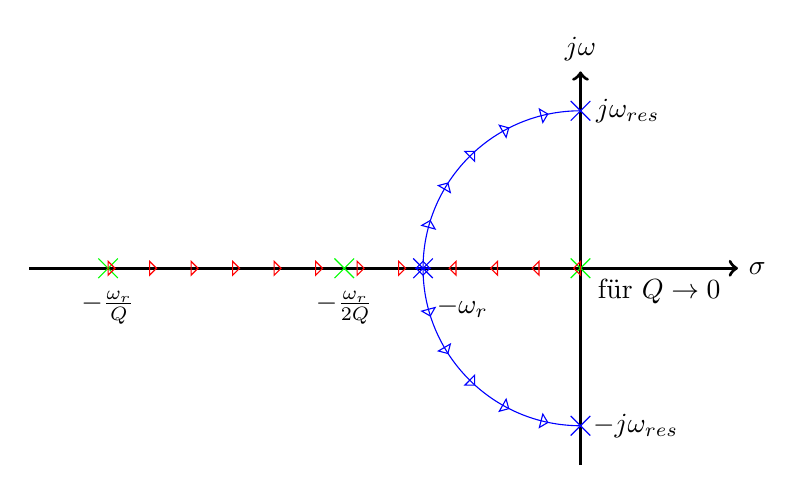
\begin{tikzpicture}
% Koordinatensystem
\begin{scope}[->, very thick]
	\draw (-7,0) -- (2,0) node[right] {$\sigma$};
	\draw (0,-2.5) -- (0,2.5) node[above] {$j\omega$};
\end{scope}

% Nullstellen
\node[cross out, draw=green] at (0,0) {} ;
\node at(1,-0.3) {für $Q \rightarrow 0$};
\node[cross out, draw=green] at (-6,0) {};
\node at(-6, -0.5) {$-\frac{\omega_r}{Q}$};
\node[cross out, draw=green] at (-3,0) {};
\node at(-3, -0.5) {$-\frac{\omega_r}{2Q}$};

% Rote Pfeile
\begin{scope}[draw=red, decoration={triangles, shape height=5, segment length=15}]
	\draw[decorate] (0,0) -- (-2,0);
	\draw[decorate] (-6,0) -- (-2,0);
\end{scope}

% Blauer Halbkreis mit Nullstelle und so.
\begin{scope}[draw=blue]
	\node[cross out, draw] at (-2,0) {};
	\node at(-1.5, -0.5) {$-\omega_r$};
	\draw (-2,0) arc (180:90:2);
	\draw (-2,0) arc (180:270:2);
	\node[cross out, draw] at (0,2) {};
	\node at (0.6, 2) {$j\omega_{res}$};
	\node[cross out, draw] at (0,-2) {};
	\node at (0.7, -2) {$-j\omega_{res}$};
\end{scope}

% Blaue Dreieckli
\begin{scope}[draw=blue, decoration={triangles, shape height=5, segment length=15}]
	\draw[decorate] (-2,0) arc (180:90:2);
	\draw[decorate] (-2,0) arc (180:270:2);
\end{scope}
\end{tikzpicture}
  \caption{Zusammenhang Güte - Frequenz}
  \label{fig:elNetzw:GueteFrequenz}
\end{center}
\end{figure}

\subsection{Zusammenhang P-N-Verteilung $\leftrightarrow$ Frequenzgang}
$\underline{F}(p)=K\frac{(p-\underline{z}_1)(p-\underline{z}_2)\ldots}{(p-p_1)(p-p_2)\ldots}$\\

\begin{figure}[!ht]
\begin{center}
  \usetikzlibrary{shapes}
\usetikzlibrary{decorations.shapes}
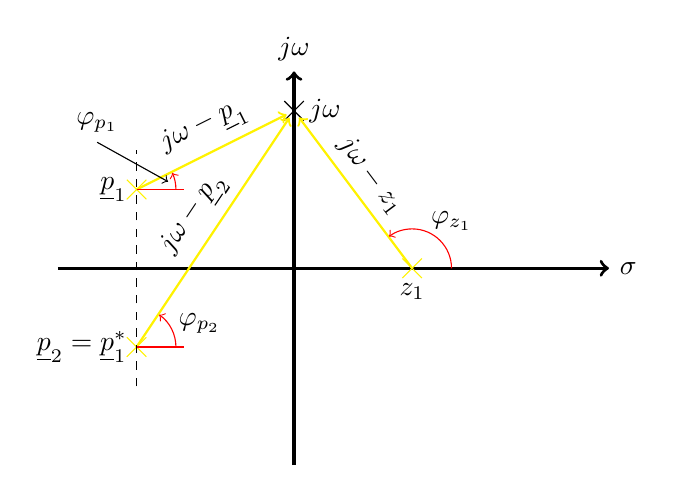
\begin{tikzpicture}

% Koordinatensystem
\begin{scope}[->, very thick]
  \draw (-3,0) -- (4,0) node[right] {$\sigma$};
  \draw (0,-2.5) -- (0,2.5) node[above] {$j\omega$};
\end{scope}

% Punkte p1, p2, z1, jw
\draw (-2,1) node[cross out, draw=yellow] {} node[left] {$\underline{p}_1$};
\draw (-2,-1) node[cross out, draw=yellow] {} node[left] {$\underline{p}_2 = \underline{p}_1^*$};
\draw (1.5,0) node[cross out, draw=yellow] {} node[below=2] {$z_1$};
\draw (0,2) node[cross out, draw] {} node[right=2] {$j\omega$};

% Linien zu jw
\begin{scope}[yellow, ->, thick, shorten >= 3pt]
  \draw (-2,1) -- (0,2) node[midway,above, sloped, black] {$j\omega -\underline{p}_1$};
  \draw (-2,-1) -- (0,2) node[midway, above, sloped, black] {$j\omega - \underline{p}_2$};;
  \draw (1.5,0) -- (0,2) node[midway,above, sloped, black] {$j\omega - z_1$};;
\end{scope}

% Winkel und Beschriftung
\begin{scope}[draw=red]
  \draw (-2,1) -- +(0.6,0); 
  \draw (-2,-1) -- +(0.6,0);
  \begin{scope}[->]
    \draw (-1.5,1) arc (0:25:0.5);
    \draw (-1.5,-1) arc (0:55:0.5);
    \draw (2,-0) arc (0:126:0.5);
  \end{scope}
\end{scope}

\draw (-1.2, -0.7) node {$\varphi_{p_2}$};
\draw (2, 0.6) node {$\varphi_{z_1}$};
\draw[<-] (-1.6,1.1) -- (-2.5,1.6) node[above] {$\varphi_{p_1}$};

% Linie p1, p2
\draw[dashed, very thin]  (-2,-1.5) -- +(0,3);
\end{tikzpicture}
  \caption{Zusammenhang Pol/Nullstellen - Frequenz}
  \label{fig:elNetzw:PNFrequenz}
\end{center}
\end{figure}

\begin{align}
	\text{Frequenzgang} p&=j\omega\nonumber\\
	\underline{F}(j\omega)&=K\frac{(j\omega-\underline{z}_1)(j\omega-\underline{z}_2)\ldots}{(j\omega-p_1)(j\omega-p_2)\ldots}\nonumber\\
	|\underline{F}(j\omega)|&=|K|\frac{\overbrace{|j\omega-\underline{z}_1|}^{c_{z1}}\overbrace{|j\omega-\underline{z}_2|}^{c_{z2}}\ldots}{\underbrace{|j\omega-p_1|}_{c_{p1}}\underbrace{|j\omega-p_2|}_{c_{p2}}\ldots}\nonumber\\
	\text{Amplitudengang}F(j\omega)&=|K|\frac{\prod_{i=1}^{n}|c_{zi}|}{\prod_{i=1}^{m}|c_{pi}|} \nonumber\\
	\text{Phasengang}\varphi =
arg\left(\underline{F}(j\omega)\right)&=\left(\varphi_{z1}+\varphi_{z2}+\ldots-\varphi_{p1}-\varphi_{p2}-\ldots\right)\nonumber\\
	\varphi &= \sum_{i=1}^n\varphi_{zi}-\sum_{i=1}^m\varphi_{pi}+k\pi\nonumber
\end{align}\\
Eine Nullstelle auf der $j\omega$-Achse bewirkt einen Phasensprung von $\pi$.\\
$\tau_{Gr}=-\frac{d}{d\omega}arg\underline{F}(j\omega)$ Gruppenlaufzeit\\
\subsection{Übersicht Netzwerke/Systeme, Lernziele}
\begin{itemize}
  \item Dualität
  \item Komplexe Frequenz
  \item Netzwerkfunktionen
  \begin{itemize}
    \item Summenform
    \item Produkform $\rightarrow$ P-N-Diagramm
    \item in Partialbrüche zerlegt
	\end{itemize}
	\item Zusammenhänge\\
	%TODO kraafick von dem?
	F(p), DGL, P-N-Plan, Frequenzgang, freie Schwingung <-- alle sind verknüpft
\end{itemize}	